
\documentclass[12pt,a4paper]{article}

\usepackage[utf8]{inputenc}
\usepackage[T1]{fontenc}
\usepackage{polski}

\usepackage{amsthm}
\usepackage{amsmath}
\usepackage{amsfonts}
\usepackage{amssymb}
\usepackage{pgfplots}
\usepackage{tikz}
\usepackage{lmodern}	%fancy font
\usepackage{textcomp}

\usepackage{indentfirst}
\usepackage{graphicx}
\usepackage{caption}
\usepackage{subcaption}
%\usepackage{siunitx}
\usepackage{here}


\setlength{\textheight}{24cm}
\setlength{\textwidth}{15.92cm}
\setlength{\footskip}{10mm}
\setlength{\oddsidemargin}{0mm}
\setlength{\evensidemargin}{0mm}
\setlength{\topmargin}{0mm}
\setlength{\headsep}{5mm}
\usepackage{tikz}
\usepackage{lmodern}	%fancy font
\usepackage{textcomp}

\usepackage{indentfirst}
\usepackage{graphicx}
\usepackage{caption}
\usepackage{subcaption}
%\usepackage{siunitx}
\usepackage{here}
\usepackage[margin=1in]{geometry}% Just for this example
\setlength{\parindent}{0pt}% Just for this example
\setlength{\textheight}{24cm}
\setlength{\textwidth}{15.92cm}
\setlength{\footskip}{10mm}
\setlength{\oddsidemargin}{0mm}
\setlength{\evensidemargin}{0mm}
\setlength{\topmargin}{0mm}


\begin{document}

\begin{table}[]
\label{my-label}
\begin{tabular}{|p{7.5cm}|p{7.5cm}|}
\hline
									           					&                           \\

\includegraphics[height=3cm]{logo}             					& \textbf{Technika cyfrowa} \\ \hline
\multicolumn{1}{|l|}{\textbf{Temat ćwiczenia}} 					& \textbf{Numer ćwiczenia}  \\
\multicolumn{1}{|l|}{Liczniki}	& 2                         \\ \hline
\multicolumn{1}{|l|}{\textbf{Wykonawca}}       & \textbf{Ocena}            \\
\multicolumn{1}{|l|}{Marcin Przewięźlikowski}          &                           \\ \hline
\end{tabular}
\end{table}

\section{Cel ćwiczenia}

Zapoznanie się z zastosowaniem przerzutników w budowaniu liczników synchronicznych oraz asynchronicznych. Zbadanie działania liczników czterobitowych.

\section{Dwójka licząca}


Dwójka licząca służy do dzielenia częstotliwości sygnału wejściowego przez 2. Uzyskano ją na dwa sposoby:

\subsection{Przerzutnik D}


Dwójka licząca służy do dzielenia częstotliwości sygnału wejściowego przez 2. Oto jej tabela prawdy:



\begin{figure}[H]
\centering
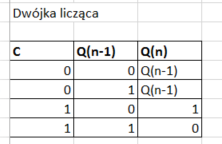
\includegraphics{img/4a_table}
\end{figure}

Uzyskano ją na dwa sposoby:

\begin{figure}[H]
\centering
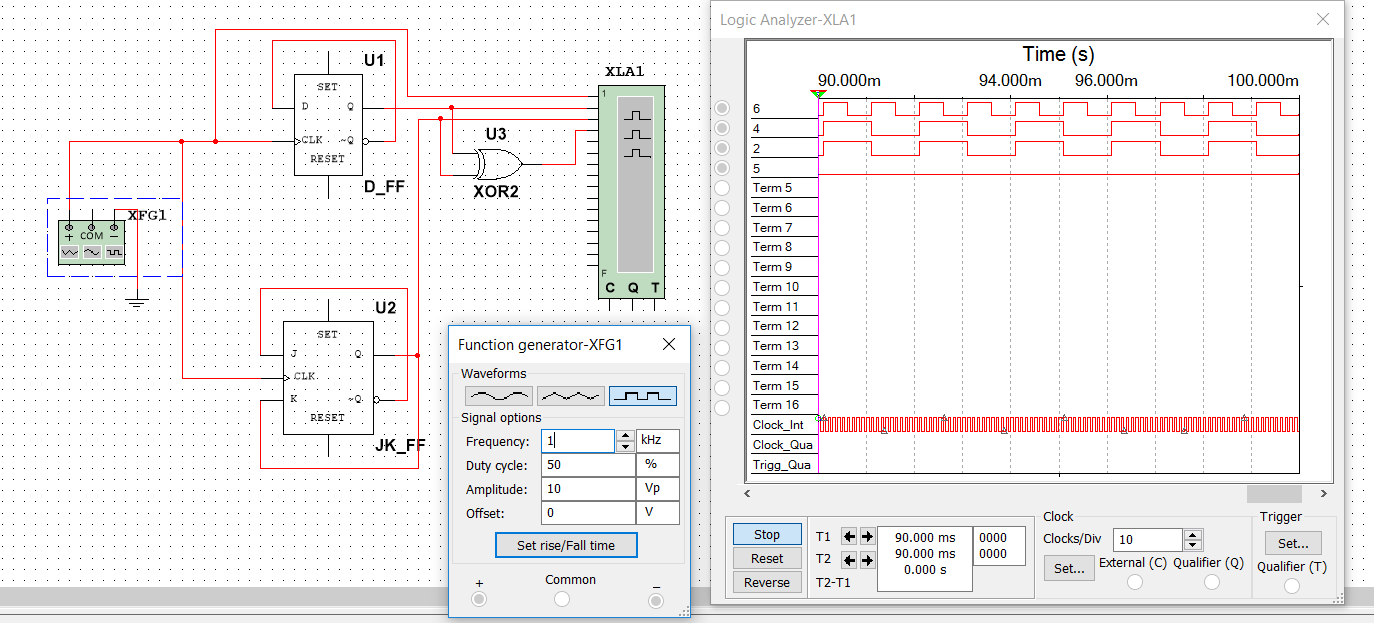
\includegraphics[width=\textwidth]{img/4a}
\end{figure}

\subsection{Przerzutnik D}
\begin{figure}[H]
\centering
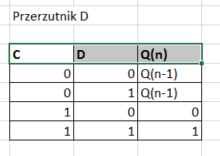
\includegraphics{img/4a_table_d}
\end{figure}
Chcemy, aby wartość logiczna Q zmieniała się na przeciwną niż dotychczasowa tylko, gdy sygnał zegara jest wzrastający.

Właściwości przerzutnika D, pozwalają na uzyskanie zmiany wartości wyjścia na wartość podaną na wejście D tylko, gdy sygnał zegara jest wzrastający. Jak jednak uzyskać zmianę sygnału na wręcz przeciwny? 
Na wejście D trzeba podać zanegowanie obecnej wartości sygnału Q - czyli -Q.

\subsection{Przerzutnik JK}

\begin{figure}[H]
\centering
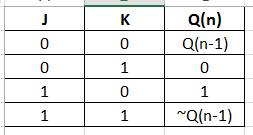
\includegraphics{img/4a_table_jk}
\end{figure}

Wyjście przerzutnika JK zmienia swój stan tylko wtedy, gdy sygnał zegara jest wzrastający. Ponadto, sygnał wyjściowy jest ustawiany zawsze na wartość wejścia J, gdy na wejścia J i K są podane przeciwne sygnały. 

W związku z tym wystarczy na wejście K podać sygnał wyjściowy (Q), a na wejście J - zanegowany sygnał wyjściowy (-Q). Mamy wtedy gwarancję, że sygnał przerzutnika zmieni się na wartość przeciwną do dotychczasowej.

\section{Czterobitowy licznik asynchroniczny}

Do budowy czterobitowego licznika użyto dwójek liczących stworzonych za pomocą przerzutników typu T ze stale podanym na wejście T sygnałem dodatnim. Sprawia to, że przerzutniki reagują zmianą sygnału wyjściowego na wzrastający sygnał zegara.
\par
Tym sposobem każdy licznik dzieli częstotliwość sygnału otrzymywanego na wyjściu C przez 2. 

\begin{figure}[H]
\centering
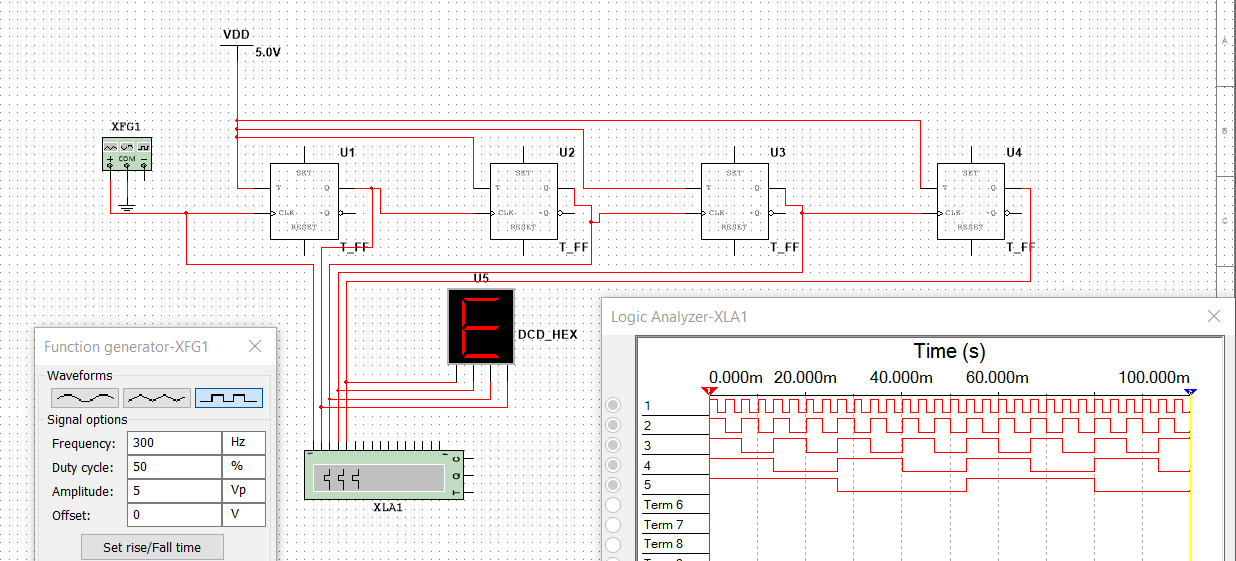
\includegraphics[width=\textwidth]{img/4b_wzrost}
\end{figure}

Zauważono następującą zależność sygnałów na wyjściu od liczby sygnałów z zegara na wejściu:

\begin{figure}[H]
\centering
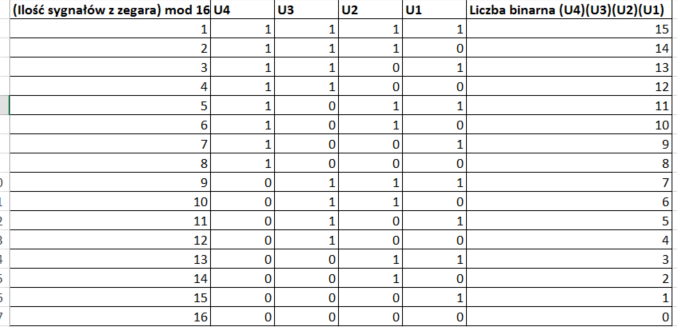
\includegraphics[width=\textwidth]{img/4b_wzrost_table}
\end{figure}

- liczba na wyjściu jest równa 16 - (liczba sygnałów z zegara mod 16) - a więc jest to licznik liczący w tył.
\par
\par 
Zrealizowano także układ w oparciu o dwójki liczące reagujące na sygnał opadający z zegara. W tym celu na wejście każdego z przerzutników T w układzie dodano bramkę NOT. 
Wtedy, gdy na wejściu bramki NOT jest sygnał opadający, podaje ona sygnał wzrastający na wejście przerzutnika T, na który ten reaguje. Efektywnie Układ NOT-T zachowuje się jak bramka T reagująca na sygnał opadający. Tak działająca bramka T również dzieli częstotliwość podanego sygnału przez 2.


\begin{figure}[H]
\centering
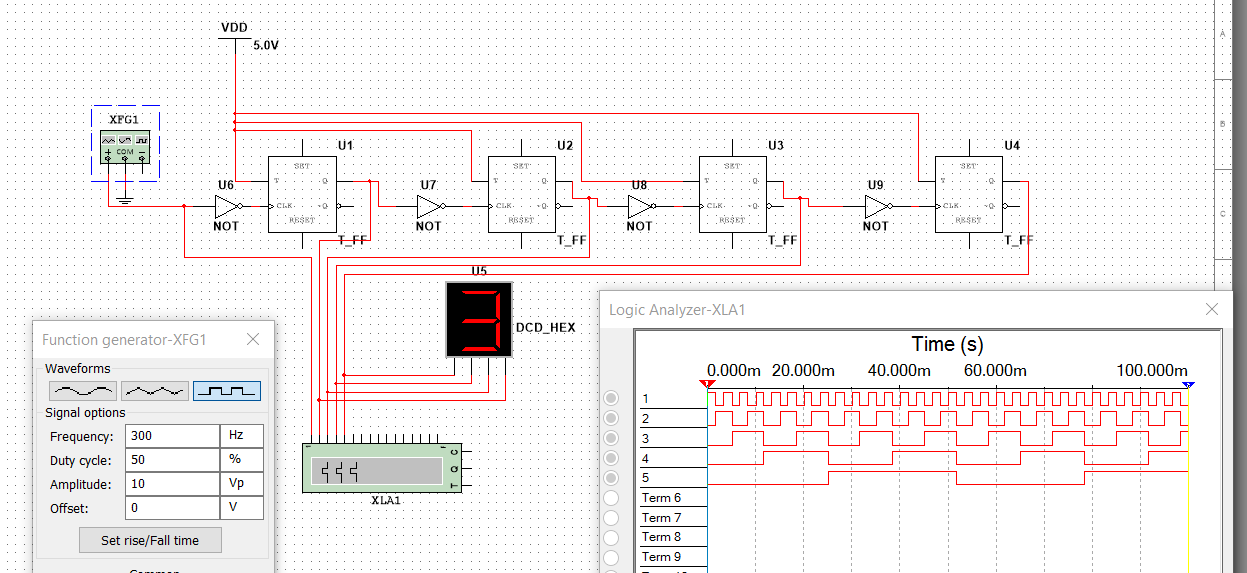
\includegraphics[width=\textwidth]{img/4b_opad}
\end{figure}

Zauważono następującą zależność sygnałów na wyjściu od liczby sygnałów z zegara na wejściu:
\begin{figure}[H]
\centering
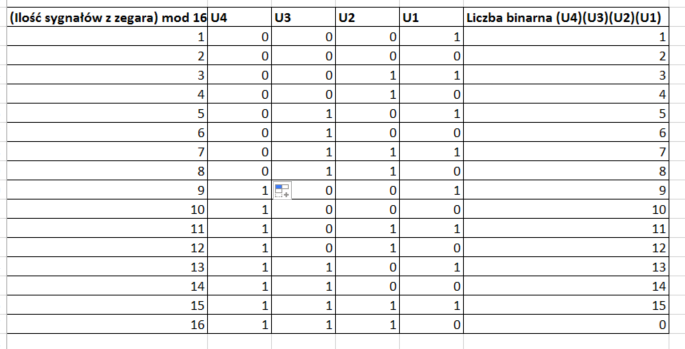
\includegraphics[width=\textwidth]{img/4b_opad_table}
\end{figure}

Widać zatem, że liczba na wyjściu jest równa liczbie sygnałów z zegara mod 16 - jest to licznik liczący w przód.

\par
Licznik ten nazywamy asynchronicznym, gdyż jego wyjście nie ustala się równocześnie z wejściem, lecz zależy od czasu propagacji sygnału w składowych przerzutnikach. Nie jest to dobre rozwiązanie - jeśli przerzutniki mają duży czas propagacji sygnału, licznik może "gubić" niektóre bity wyjścia lub też po prostu podawać niewłaściwy ich zestaw.

\section{Synchroniczny licznik mod 8}

Liczniki synchroniczne rozwiązują problem liczników asynchronicznych - sygnał zegara jest podawany na każdy z przerzutników osobno, zatem redukuje się czas opóźnień.

Ponieważ licznik jest modulo 8, to wystarczy, by jego wyjście było 3-bitowe.

Rozważmy tabelę prawdy dla każdego z wyjść licznika:

\begin{figure}[H]
\centering
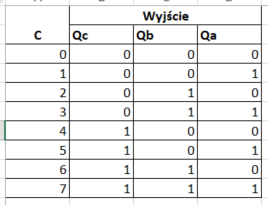
\includegraphics{img/4c_table}
\end{figure}

Na tej podstawie można stworzyć tabele Karnaugh'a dla funkcji logicznych sterujących przerzutnikami D.
Przypomnijmy, że wyjście przerzutnika D przyjmuje wartość sygnału podanego na wejście D, gdy na wejście zegarowe podany jest sygnał wysoki.
W poniższych tabelach przez Qc, Qb i Qa rozumiemy wartości tych wyjść przy poprzednim sygnale zegara:
 

\begin{figure}[H]
\centering
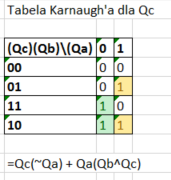
\includegraphics{img/4c_table_qc}
\end{figure}

\begin{figure}[H]
\centering
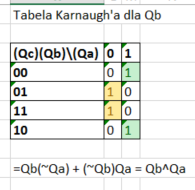
\includegraphics{img/4c_table_qb}
\end{figure}

\begin{figure}[H]
\centering
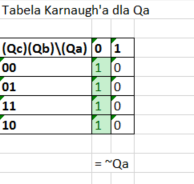
\includegraphics{img/4c_table_qa}
\end{figure}

Na podstawie uzyskanych funkcji logicznych zrealizowano następujący układ, w którym wejścia D przerzutników są sterowane uzyskanymi funkcjami:


\begin{figure}[H]
\centering
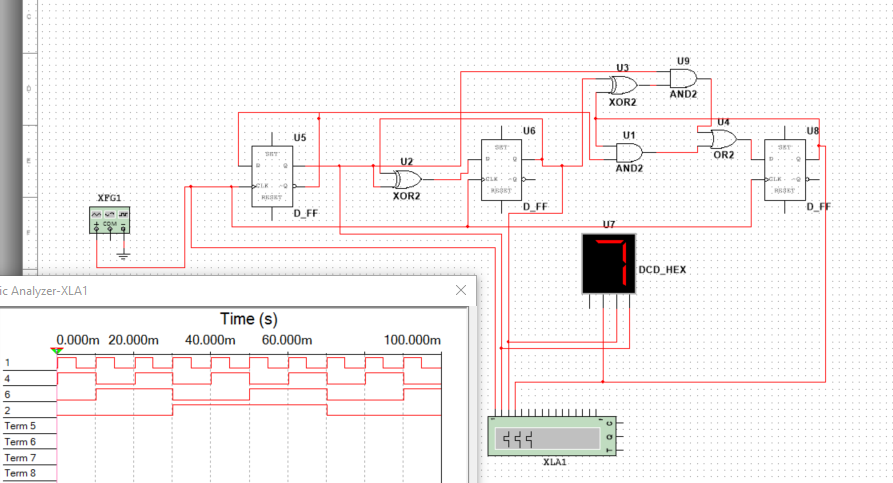
\includegraphics[width=\textwidth]{img/4c}
\end{figure}

\section{Synchroniczny licznik mod 6}
Mając synchroniczny licznik mod 8, zrealizowanie licznika mod 6 nie jest dużym wyzwaniem. Zgodnie z tabelą prawdy dla tego licznika:

\begin{figure}[H]
\centering
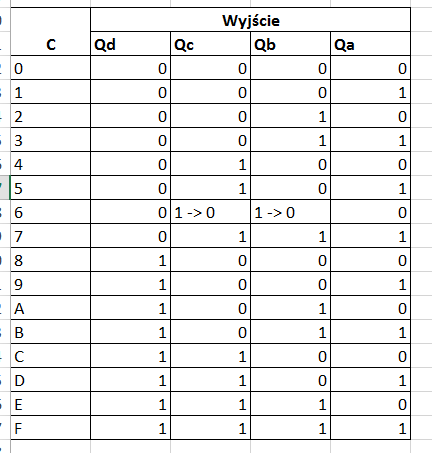
\includegraphics{img/4d_table}
\end{figure}

Wszystkie przerzutniki muszą zostać wyzerowane, gdy na wyjściach Qc i Qb pojawią się sygnały dodatnie. Aby to zrealizować, do schematu licznika modulo 8 dodano małą modyfikację - zerowanie przerzutników sygnałem z bramki AND łączącej Qc i Qb:

\begin{figure}[H]
\centering
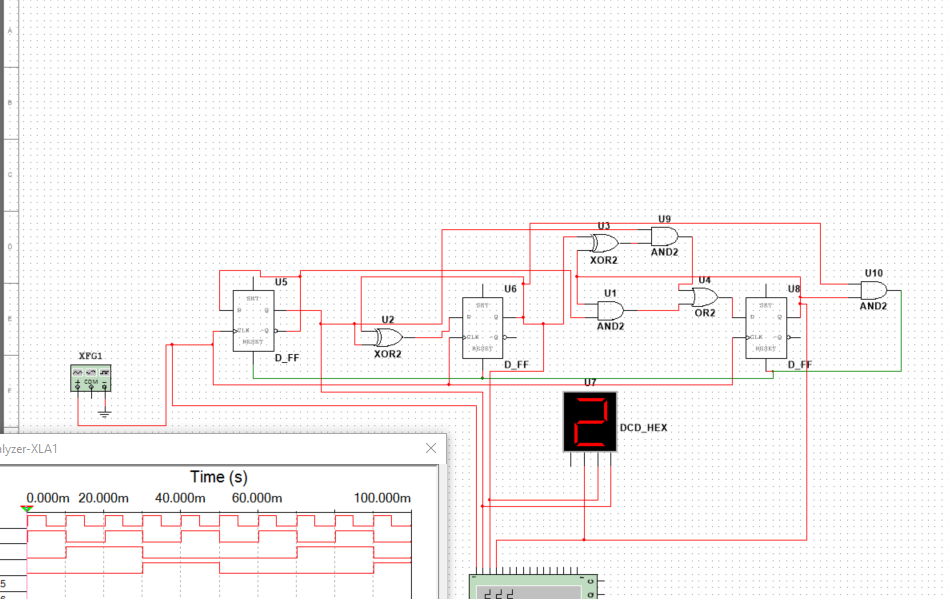
\includegraphics[width=\textwidth]{img/4d}
\end{figure}


\section{Synchroniczny licznik mod (dowolna 3-bitowa liczba)}

Wykorzystując zasadę działania licznika mod 6, zrealizowano licznik, który zwraca resztę z dzielenia liczby taktów zegara przez dowolną 3-bitową liczbę. Wykorzystano do tego 3 bramki XNOR połączone bramką AND3, które efektywnie zwracają wartość logiczną 1, gdy odpowiednie podane na ich wejścia pary bitów są sobie równe. Dzięki temu można zerować przerzutniki D, gdy osiągniemy wybraną przez nas liczbę. Licznik przetestowano wyświetlaczami siedmiosegmentowymi i stwierdzono jego poprawne działanie. 

\begin{figure}[H]
\centering
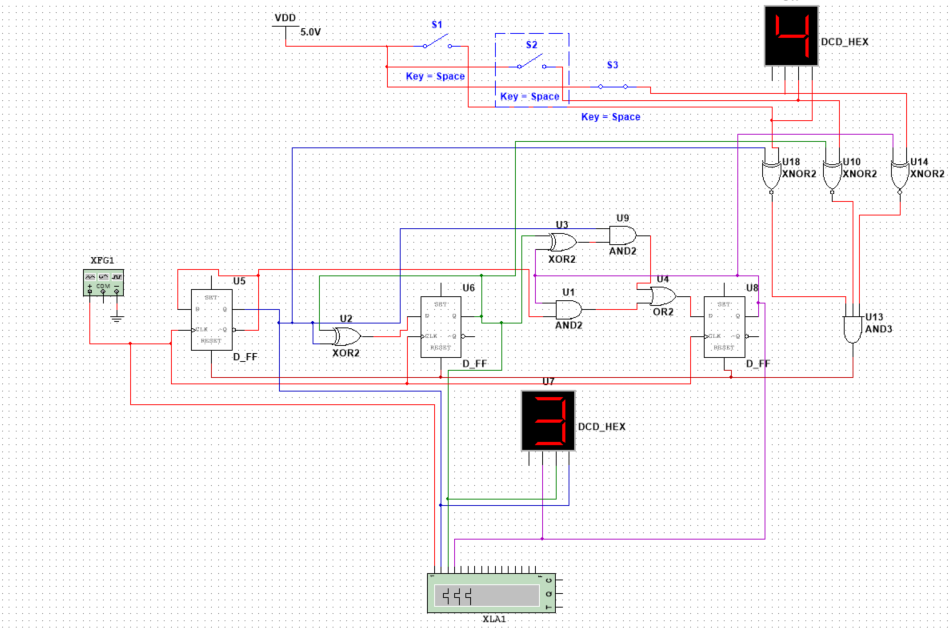
\includegraphics[width=\textwidth]{img/4extra}
\end{figure}

Konstrukcja ta jest mniej optymalna jeśli chodzi o wykorzystaną liczbę bramek logicznych od liczników z odgórnie zdefiniowaną liczbą, przez którą dzielą - jest ona jednak ogólniejsza w swoim działaniu.



\end{document}
